\begin{figure}
  \centering
  % Requires \usepackage{graphicx}
  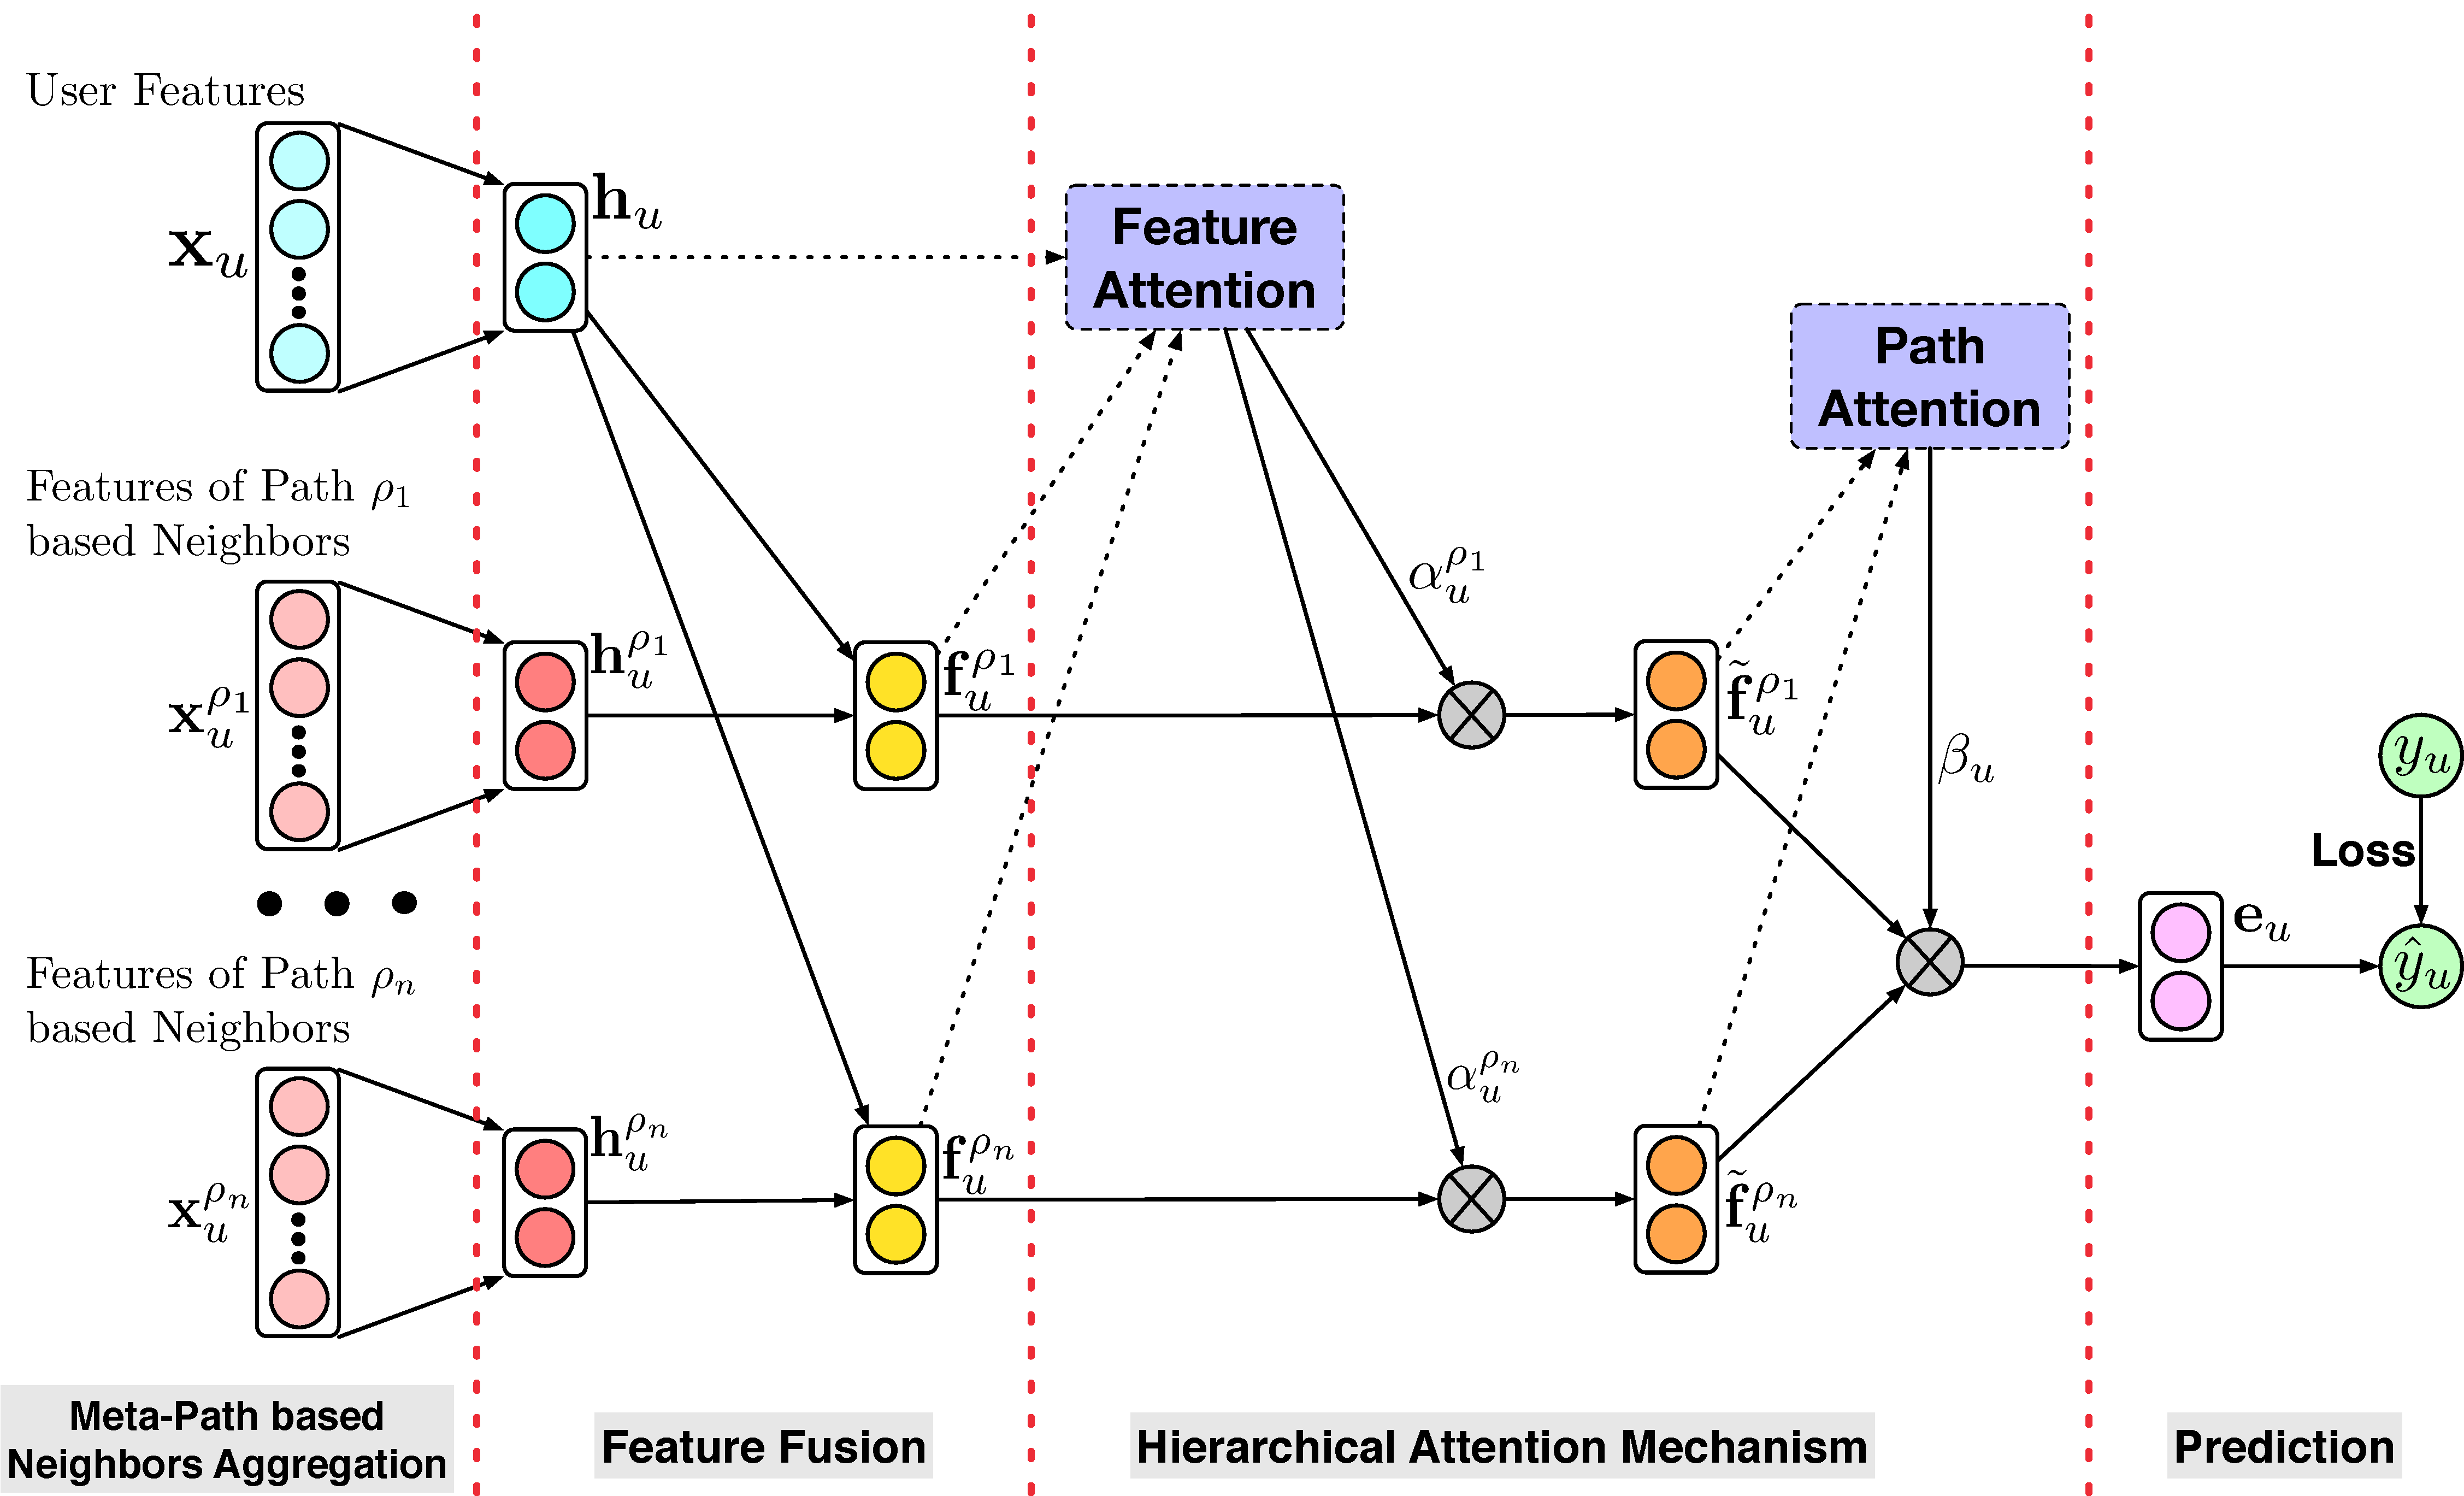
\includegraphics[width=8.5cm]{image/Model_Attention.pdf}\\
  \caption{The architecture of the proposed model}\label{fig-model}
\end{figure}

\section{The Proposed Model}
In this section, we firstly analyze the effect of meta-path based neighbors on the cash-out user detection on real data and then present the proposed \emph{\textbf{H}ierarchical \textbf{A}ttention mechanism based \textbf{C}ash-out \textbf{U}ser \textbf{D}etection model}, called \textbf{HACUD} shortly.
We show the overall architecture of the proposed model in Fig.~\ref{fig-model}. Firstly, we aggregate neighbors for each user based on different meta-paths to integrate multiple aspects of structure information in AHIN, and then we transform and fuse the original features for better representation learning. Considering that different features and meta-paths have different importances, we design a hierarchical attention mechanism to model user preferences towards features and meta-paths. %Due to the integration of meta-path and attribute based information in AHIN, our model is expected to yield a better performance in cash-out user detection problem.

\begin{figure}[t]
\centering
\subfigure[UMU]{
  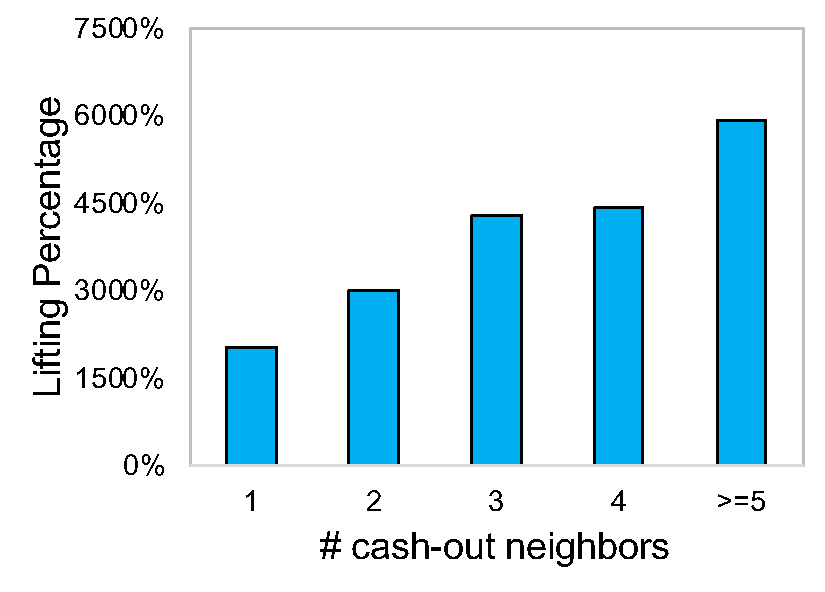
\includegraphics[width=4.0cm]{image/network_analysis_1.pdf}\label{fig:network1}}
\subfigure[UU]{
  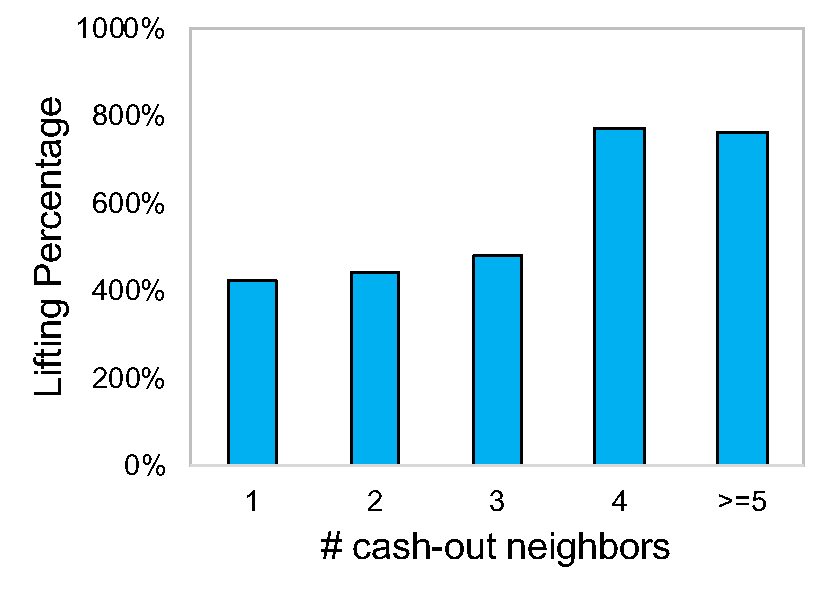
\includegraphics[width=4.0cm]{image/network_analysis_3.pdf}\label{fig:network3}}
%\subfigure[UMDMU]{
%  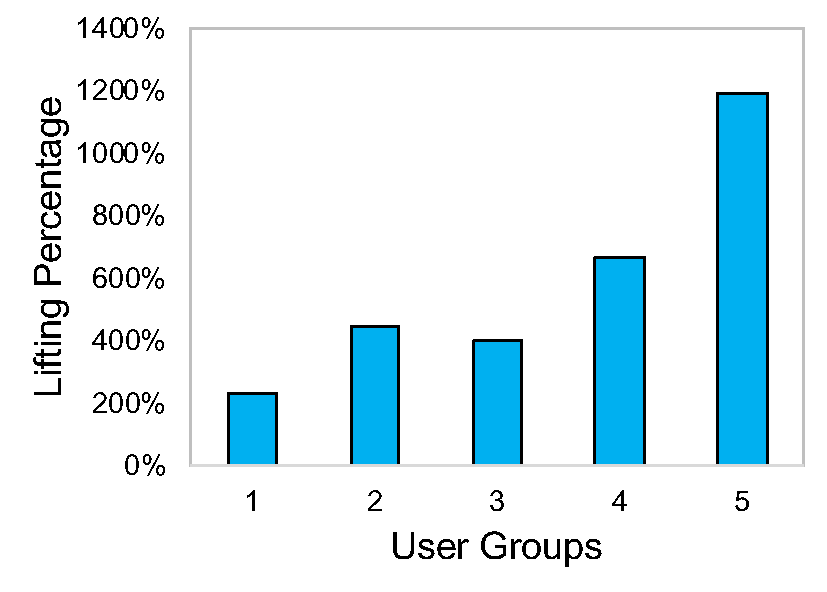
\includegraphics[width=5.6cm]{image/network_analysis_2.pdf}\label{fig:network2}}
\caption{The lifting percentages of cash-out rate in users with different amount of cash-out neighbors against users without any cash-out neighbor in two meta-paths.}%To be noted that the above results are calculated based on the real world dataset from Ant Credit Pay, an online credit payment service provided by Ant Financial Services Group.}
\label{fig:network_analysis}
\end{figure}

\subsection{Observations in Real Data}
Intuitively, the cash-out users tend to aggregate closely through different kinds of interactions.
Taking the AHIN in Fig. \ref{fig-hin} as an example, cash-out users tend to make more transactions with merchants which sell particular goods (e.g., pre-pard cards) or interact with more deceivers. 
In order to validate the aggregation of cash-out users with respect to different relations, we do experiments on the real dataset in Ant Credit Pay of Ant Financial Services Group (see Ten Days Dataset in Experiments). 

We first collect the meta-path based neighbors of each user based on two meta-paths ($UMU$ meaning users having transactions with the same merchants and $UU$ meaning users having fund transfer from one to another). 
For each meta-path, we count the number of neighbors who are cash-out user (called cash-out neighbor), and divide all users into different groups with respect to the number of their cash-out neighbors.
The cash-out rate (i.e., the proportion of cash-out users) is calculated in each group. The lifting percentages of cash-out rate in different user groups against users without any cash-out neighbor, with respect to two meta-paths, are presented in Fig. \ref{fig:network_analysis}. 
We have the following observations.

(1) Users with higher cash-out rate tend to have more cash-out neighbors.
This observation illustrates that 
%meta-path neighbors have great impact on recognizing cash-out users and can be utilized  to enhance the target users' representations. 
meta-path based neighbors have consistent behaviors with the original user, which implies that the features of users can stem from that of their meta-path based neighbors.

(2) Different meta-path based neighbors have different impacts on users. In Fig. \ref{fig:network_analysis}, two meta-paths yield different lifting percentages. %especially for users with no less than 5 cash-out neighbors through UMU path, the cash-out rate is around 60 times larger than users without any cash-out neighbor (Fig \ref{fig:network1}). 
%It inspires us to model this problem with a hierarchical attention mechanism, which automatically learns the importance of attributes and meta-paths.
It inspires us that different meta-paths have different importances on users, which can be captured by recent emerging attention mechanism.

\subsection{Meta-path based Neighbors Aggregation}
Inspired by recently emerging graph convolutional networks~\citep{Kipf2016Semi,dai2016discriminative} and the above observations on real data, we think that feature representations of objects, besides their intrinsic features, are also composed of the features of their neighbors. Based on this idea, we aggregate meta-path based neighbors for each user. 
%To capture multiple aspect of information in AHIN, we collect neighbors based on different meta-paths. For each user $b$, we denote the neighborhood based on a meta-path $\rho$ as $\mathcal{N}^{\rho}_u$. In order to adapt our model to large scale network, inspired by the recent progress on 
Specifically, similar to recent attributed network embedding~\citep{liang2018semi,zhang2018anrl}, we adopt to represent a node \wrt a certain meta-path via aggregating features of its neighbors rather than the one-hot representation of its neighbors. For each user $u$, we can obtain the \emph{aggregated features based on meta-path} $\rho$ as below:
\begin{equation}
\mathbf{x}^{\rho}_u = \sum_{j \in \mathcal{N}^{\rho}_u}{w^{\rho}_{uj} * \mathbf{x}_j},
\end{equation}
where $\mathcal{N}^{\rho}_u$ is the neighbors of node $j$ based on meta-path $\rho$ and $\mathbf{x}_j$ represents the attribute information vector associated with node $j$. The given link weight $w_{uj} > 0$ for weighted networks and $w_{uj} = 1$ for unweighted networks.


\subsection{Feature Fusion}
For each user $u$, we can obtain its own feature $\mathbf{x}_u$ as well as a set of its neighbor aggregation features based on multiple meta-paths $\{\mathbf{x}^{\rho}_u\}_{\rho \in \mathcal{P}}$ where $\mathcal{P}$ denotes the set of meta-paths. For better representation learning, we set up a \emph{feature fusion} part to  transform and fuse the original features. 

Firstly, we project the original sparse features to the low-dimensional dense representations, and obtain the \emph{latent representations} of user $u$ and his/her neighbors based on different meta-paths (i.e., $\mathbf{h}_u$ and $\mathbf{h}_u^\rho$), respectively: %which can be formulated as follows:
%\begin{eqnarray}
%\mathbf{h}_u &=& \mathbf{W}\mathbf{x}_u + \mathbf{b}, \\
%\mathbf{h}^{\rho}_u &=& \mathbf{W}^{\rho}\mathbf{x}^{\rho}_u + \mathbf{b}^{\rho}, %\nonumber
%\end{eqnarray}
\begin{equation}
\mathbf{h}_u = \mathbf{W}\mathbf{x}_u + \mathbf{b}, \ \ \ \ \mathbf{h}^{\rho}_u = \mathbf{W}^{\rho}\mathbf{x}^{\rho}_u + \mathbf{b}^{\rho},
\end{equation}
where $\mathbf{W}^* \in \mathbb{R}^{D \times d}$ and $\mathbf{b}^* \in \mathbb{R}^{d}$ are the weight matrix and bias vector, respectively. $D$ is the dimension of original feature space\footnote{The original attributes are discretized to sparse  $D$-dimensional feature as the model input} and $d$ is the dimension of latent representations. Next, we fuse the latent representations of a user and his/her neighbors based on each meta-path and add a fully-connected layer for more complicated interaction. For a meta-path $\rho$, we formulate the above procedure and obtain the \emph{fusional representation} $\mathbf{f}_u^{\rho}$ \wrt meta-path $\rho$ as below,
\begin{equation}
\mathbf{f}^{\rho}_u =\text{ReLU}(\mathbf{W}_{F}^{\rho}g(\mathbf{h}_u, \mathbf{h}^{\rho}_u) + \mathbf{b}^{\rho}_F).
\end{equation}
Here, $\textbf{W}_F^{\rho} \in \mathbb{R}^{d \times 2d}$ and $\mathbf{b}^{\rho}_F \in \mathbb{R}^{d}$ represent the weight matrix and bias vector based on meta-path $\rho$, respectively. $g(\cdot , \cdot)$ is the fusion function, which can be concatenation, addition or element-wise product (In our implementation, $g(\cdot , \cdot)$ is concatenation).
\subsection{Hierarchical Attention}
Intuitively, different users are likely to have different preferences over the features based on different meta-paths as well as attribute information. Concretely, a user may place different importances to different-aspect features based on meta-paths. Moreover, features also have different importances for the prediction task.
%the various aspects based on different meta-paths, and an important aspect sometimes can highly contribute to the prediction for the high risk users. Furthermore, different meta-path can also contribute to the prediction unequally since they convey different semantics. 
Due to the effectiveness of attention mechanism in various machine learning tasks~\citep{hu2018leveraging,Cheng2018A,you2016image}, we design a hierarchical attention mechanism to capture user preferences towards features and meta-paths.
\subsubsection{Feature Attention}
Since different features might not contribute to the prediction task equally, we learn the aspect-specific attention weights over features conditioned on the involved user based on each meta-path. Given the user latent representation $\mathbf{h}_u$ and latent representation of his/her neighbors $\mathbf{f}^{\rho}_u$ based on meta-path $\rho$ , we adopt a two-layer neural network to implement the attention.
%\begin{equation}
%\bm{\alpha}_b^{\rho} = \text{RELU}(\mathbf{W}_f^2\text{RELU}(\mathbf{W}_f^1[\mathbf{h}_b ; \mathbf{f}_b^{\rho}] +\mathbf{b}_f^1) + \mathbf{b}_f^2),
%\end{equation}
\begin{eqnarray}
\bm{v}_u^{\rho} &=& \text{ReLU}(\mathbf{W}_f^1[\mathbf{h}_u ; \mathbf{f}_u^{\rho}] +\mathbf{b}_f^1), \\
\bm{\alpha}_u^{\rho} &=& \text{ReLU}(\mathbf{W}_f^2\bm{v}_u^{\rho} + \mathbf{b}_f^2),
\end{eqnarray}
where $\mathbf{W}_f^*$ and $\mathbf{b}_f^*$ denote the weight matrix and bias vector, respectively and $[\cdot ; \cdot]$ represents the concatenation of two vectors. Following the standard setting of neural attention networks, we normalize the above attention scores with the softmax function to obtain the final attention weights.
\begin{equation}
\hat{\alpha}_{u, i}^{\rho} = \frac{\exp(\alpha_{u, i}^{\rho})}{\sum_{j = 1}^{K}{\exp(\alpha_{u, j}^{\rho})}}.
\end{equation}
Then, the final representation of user $u$ \wrt a meta-path $\rho$ can be computed as follows,
\begin{equation}
\label{equ-f-tilde}
\widetilde{\mathbf{f}}^{\rho}_u = \bm{\hat{\alpha}}_u^{\rho} \bigodot \mathbf{f}_u^{\rho},
\end{equation}
where ``$\bigodot$'' denotes the element-wise product.
\subsubsection{Path Attention}
Given a user, following the above steps, we could obtain multiple representations based on multiple meta-paths, which are expected to collaborate with each other for better prediction. Following~\citep{qu2017attention}, we learn  the attention weights over different meta-paths for collaboration. Specifically, we define the attention weight of meta-path $\rho$ for user $u$ using a softmax unit as follows:
\begin{equation}
\beta_{u, \rho} = \frac{\exp({\mathbf{z}^{\rho}}^{\mathrm{T}} \cdot \mathbf{\widetilde{f}}^C_u)}{\sum_{\rho' \in \mathcal{P}}{\exp({\mathbf{z}^{\rho^\prime}}^{\mathrm{T}} \cdot \mathbf{\widetilde{f}}^C_u)}},
\end{equation}
where $\mathbf{z}^{\rho} \in \mathbb{R}^{|\mathcal{P}| * d}$ is the attention vector for meta-path $\rho$ and $\widetilde{\mathbf{f}}^C_u$ is the concatenation of user $u$'s representations \wrt all meta-paths ($\ie$ $\widetilde{\mathbf{f}}^{\rho}_u$). After obtaining the path attention scores $\beta_{u, \rho}$, the final representation aggregating all meta-paths is given as the following weighted sum form:
\begin{equation}
\mathbf{e}_u = \sum_{\rho \in \mathcal{P}}{\beta_{u, \rho} * \mathbf{\widetilde{f}}^{\rho}_u},
\end{equation}
where $\mathbf{\widetilde{f}}^{\rho}_u$ is the representation of neighbors for user $u$ based on meta-path $\rho$ in Eq.~\ref{equ-f-tilde}.

\subsection{Model Learning}
Since neural networks have shown strong ability in modeling the complex interactions~\citep{he2017neural}, we feed the obtained final representation (\ie $\mathbf{e}_u$) into multiple fully connected neural networks as follows,
\begin{equation}
\mathbf{z}_u = \text{ReLU}(\textbf{W}_{L} \cdots \text{ReLU}(\mathbf{W}_1\mathbf{e}_u + \mathbf{b}_1) + \mathbf{b}_{L}),
\end{equation}
where $\mathbf{W}_*$ and $\mathbf{b}_*$ respectively denote the weight matrix and the bias vector for each layer. The predicted cash-out probability is obtained via a regression layer with a sigmoid unit:
\begin{equation}
p_u = \text{sigmoid}(\mathbf{w}_p^{T}\mathbf{z}_u + b_p).
\end{equation}
Here $\mathbf{w}_p$ and $b_p$ are the weight vector and the bias, respectively. As our task is classification, we model the objective function with maximum likelihood estimation, which can be formulated as follows:
\begin{equation}
\label{equ-objective}
\mathcal{L}(\Theta) = \sum_{\langle u, y_u \rangle \in \mathcal{D}}(y_u\log(p_u) + (1 - y_u)\log(1 - p_u)) + \lambda ||\Theta||^2_2, 
\end{equation}
where $y_u$ and $p_u$ represent the ground truth and the predicted cash-out probability of user $u$, respectively. $\Theta$ is the parameter set of the proposed model and $\lambda$ is the regularizer parameter. The stochastic gradient descent (SGD) or its variants are adopted for optimization.

\subsection{Discussion}
As mentioned above, the proposed model is a flexible framework to leverage structure and attribute information through capturing multiple aspects in AHIN. Based on different meta-paths, we can integrate various kinds of heterogeneous information to enhance the prediction performance. Moreover, we represent a user via the feature aggregation of his/her neighbors based on meta-paths, which is a natural way to combine network structure and attribute information. Compared to traditional network embedding methods~\citep{wang2016structural,dai2016discriminative}, which represent nodes via their context (\eg adjacency matrix), our method is more suitable for large-scale networks. Specifically, the dimension of original input can be reduced from $\mathcal{O}(|\mathcal{V}|)$ to $\mathcal{O}(D)$, where $|\mathcal{V}|$ is the total number of nodes in network and $D$ is the feature dimension after  discretization for each user ($D \ll |\mathcal{V}|$). For a new user which never appears in training set, the proposed model can also learn the representation through his/her meta-path based neighbors in networks. Therefore, our model has the ability to give predictions dynamically to some extent.
